%%%%%%%%%%%%%%%%%%%%%%%%%%%%%%%%%%%%%%%%%
% Beamer Presentation
% LaTeX Template
% Version 1.0 (10/11/12)
%
% This template has been downloaded from:
% http://www.LaTeXTemplates.com
%
% License:
% CC BY-NC-SA 3.0 (http://creativecommons.org/licenses/by-nc-sa/3.0/)
%
%%%%%%%%%%%%%%%%%%%%%%%%%%%%%%%%%%%%%%%%%

%----------------------------------------------------------------------------------------
%	PACKAGES AND THEMES
%----------------------------------------------------------------------------------------

\documentclass{beamer}


\mode<presentation> {

% The Beamer class comes with a number of default slide themes
% which change the colors and layouts of slides. Below this is a list
% of all the themes, uncomment each in turn to see what they look like.

\usetheme{default}

\usefonttheme{serif} % default family is serif

%\usetheme{AnnArbor}
%\usetheme{Antibes}
%\usetheme{Bergen}
%\usetheme{Berkeley}
%\usetheme{Berlin}
%\usetheme{Boadilla}
%\usetheme{CambridgeUS}
%\usetheme{Copenhagen}
%\usetheme{Darmstadt}
%\usetheme{Dresden}
%\usetheme{Frankfurt}
%\usetheme{Goettingen}
%\usetheme{Hannover}
%\usetheme{Ilmenau}
%\usetheme{JuanLesPins}
%\usetheme{Luebeck}
%\usetheme{Madrid}
%\usetheme{Malmoe}
%\usetheme{Marburg}
%\usetheme{Montpellier}
%\usetheme{PaloAlto}
%\usetheme{Pittsburgh}
%\usetheme{Rochester}
%\usetheme{Singapore}
%\usetheme{Szeged}
%\usetheme{Warsaw}

% As well as themes, the Beamer class has a number of color themes
% for any slide theme. Uncomment each of these in turn to see how it
% changes the colors of your current slide theme.

%\usecolortheme{albatross}
%\usecolortheme{beaver}
%\usecolortheme{beetle}
%\usecolortheme{crane}
%\usecolortheme{dolphin}
%\usecolortheme{dove}
%\usecolortheme{fly}
%\usecolortheme{lily}
%\usecolortheme{orchid}
%\usecolortheme{rose}
%\usecolortheme{seagull}
%\usecolortheme{seahorse}
%\usecolortheme{whale}
%\usecolortheme{wolverine}

%\setbeamertemplate{footline} % To remove the footer line in all slides uncomment this line
%\setbeamertemplate{footline}[page number] % To replace the footer line in all slides with a simple slide count uncomment this line

%\setbeamertemplate{navigation symbols}{} % To remove the navigation symbols from the bottom of all slides uncomment this line
}

\usepackage{graphicx} % Allows including images
\usepackage{booktabs} % Allows the use of \toprule, \midrule and \bottomrule in tables
\usepackage{multicol}
\usepackage{scrextend}
\usepackage{subfig}

\newcommand{\dd}{\mathrm{d}}
\newcommand{\thetaxy}{\theta_{X|Y }}
\newcommand{\thetayx}{\theta_{Y|X}}

\newcommand{\Nxy}{{N_{X|Y}}}
\newcommand{\Nyx}{{N_{Y|X}}}
\newcommand{\Nyy}{{N_{Y|Y}}}
\newcommand{\Nxx}{{N_{X|X}}}

\newcommand{\dxy}{{\delta_{X|Y}}}
\newcommand{\dyx}{{\delta_{Y|X}}}
\newcommand{\dyy}{{\delta_{Y|Y}}}
\newcommand{\dxx}{{\delta_{X|X}}}
\newcommand{\X}{\textcolor{red}{X}}
\newcommand{\Y}{\textcolor{blue}{Y}}

\definecolor{darkpurple}{rgb}{0.4,0.,0.4}

\usepackage{tcolorbox}

\definecolor{mycolor}{rgb}{0.122, 0.435, 0.698}

\usepackage{tcolorbox}
\newtcolorbox{mybox}{colback=mycolor!5!white,colframe=mycolor!75!black}




\newtcolorbox{mybox1}[1]{colback=blue!5!white,colframe=blue!75!black,fonttitle=\bfseries,title=#1}

\newtcolorbox{mybox2}[1]{colback=green!5!white,colframe=green!75!black,fonttitle=\bfseries,title=#1}

\newtcolorbox{mybox3}[1]{colback=red!5!white,colframe=red!75!black,fonttitle=\bfseries,title=#1}


\usepackage{multimedia}    
\usepackage{lipsum}


%\usepackage[hang,small]{caption}
%----------------------------------------------------------------------------------------
%	TITLE PAGE
%----------------------------------------------------------------------------------------

%\title[Short title]{Eigenfunction expansion of the refractory density for renewal processes} % The short title appears at the bottom of every slide, the full title is only on the title page

\title[Short title]{Low-dimensional population dynamics of spiking neurons via eigenfunction expansion}


\author{No\'e Gallice \\ \medskip Professor: Wulfram Gerstner \hspace{0.5cm}  Supervisor: Tilo Schwalger} % Your name
\institute[EPFL] % Your institution as it will appear on the bottom of every slide, may be shorthand to save space
{ Laboratory of Computational Neuroscience, EPFL \\ % Your institution for the title page
\medskip % Your email address
}
% Date, can be changed to a custom date
\date{April 12, 2018}

\titlegraphic{
\includegraphics[width=2.5cm]{epfl}\hspace*{4.75cm}~%
	
\includegraphics[width=2cm]{lcn}
}

\begin{document}

\begin{frame}
	\titlepage % Print the title page as the first slide
\end{frame}


\begin{frame}

\small{
	\begin{columns}
	\begin{column}{.12\textwidth}

		
	\end{column}
	\begin{column}{.28\textwidth}
			\centering
		\textbf{Complex system } 
		
	\end{column}
	\begin{column}{.3\textwidth}
			\centering
\textbf{Simplified model} 
	
\end{column}
	\begin{column}{.3\textwidth}
			\centering
		\textbf{Math. tractable / comput. efficiency}
	\end{column}
\end{columns}

\vspace{0.5cm}

\begin{columns}
	\begin{column}{.15\textwidth}
		\textit{Neuron:}
		
	\end{column}
	\begin{column}{.25\textwidth}
	\centering
	Biophysical model 	
	\end{column}
	\begin{column}{.3\textwidth}
	\centering
	Hodgkin-Huxley model 
	\end{column}
	\begin{column}{.3\textwidth}
	\centering
	IF model
	\end{column}
\end{columns}

\pause
\vspace{0.5cm}
\begin{columns}
	\begin{column}{.15\textwidth}
		\textit{Neuronal network:} 
		
	\end{column}
	\begin{column}{.25\textwidth}
		\centering
	Spiking network
	\end{column}
	\begin{column}{.3\textwidth}
		\centering
	  Population density equation
	\end{column}
	\begin{column}{.3\textwidth}
		\centering
		\textcolor{red}{Firing rate model}
	\end{column}
\end{columns}
}

\pause
\vspace{1.2cm}
M. Mattia, P. Del Giudice,  \textit{Phys. Review} (2002)

They derived a low dynamics of the collective firing rate from the spectral expansion of the Fokker-Plank equation.

\vspace{0.8cm}
\pause
\begin{mybox}
	\textbf{Aim: } Derive a low dimensional dynamics taking into account the slowest modes of the expansion of the refractory density.

\end{mybox}

\end{frame}



\begin{frame}
\frametitle{Overview}% Table of contents slide, comment this block out to remove it
\tableofcontents % Throughout your presentation, if you choose to use \section{} and \subsection{} commands, these will automatically be printed on this slide as an overview of your presentation
\end{frame}

%----------------------------------------------------------------------------------------
%	PRESENTATION SLIDES
%----------------------------------------------------------------------------------------

%------------------------------------------------




\setbeamerfont{framesubtitle}{size=\normalsize }

\section{1. Refractory density $q(\tau,t)$}
\subsection{1.1 Refractory density equation}
\subsection{1.2 The refractory density for a LIF neuron }


\begin{frame}
\frametitle{1. Refractory density $q(\tau,t)$}
\framesubtitle{1.1 Refractory density equation}
%We consider a large homogeneous population of neurons modeled by a time dependent renewal process. 

In a large homogeneous population of neurons, spikes are generated at time $t$ according to a hazard function $\rho(t,\tau)$

\vspace{0.3cm}
\pause
The state variable $\tau$ is the age of the neuron.

\vspace{0.3cm}
\pause
The refractory density $q(\tau,t)$ obeys the master equation:

\vspace{0.3cm}
\hspace{2.5cm}$
\partial_t q(\tau,t)=-\partial_\tau q(\tau,t)-\rho(\tau,t)q(\tau,t)
$

\pause
\vspace{0.3cm}
With boundary conditions:
\begin{align}
\label{boundarycondition}
q(0,t)&=\int_{0}^{\infty}\rho(\tau,t)q(\tau,t)d\tau=A(t) \nonumber\\
q(\infty,t)&=0 \nonumber
\end{align}

\end{frame}


\begin{frame}
\frametitle{1. Refractory density $q(\tau,t)$}
\framesubtitle{1.2 The refractory density for a LIF neuron}
The hazard function for a LIF neuron with exponential link function is:

\vspace{0.1cm}
\hspace{3cm}$\rho(\tau,t)=C\exp(\frac{u(\tau,t)-V_{th}}{\Delta})$

\vspace{0.4cm}
with membrane potential:

\vspace{0.1cm}
\hspace{1.6cm} $u(\tau,t)=V_r e^{-\tau/\tau_m}+\frac{1}{\tau_m}\int_0^\tau  e^{-s/\tau_m}\mu(t-s))ds$

\vspace{0.4cm}
where $\mu(t)$ is a time dependent input current, $V_r$ is a reset potential and $\Delta$ sets the sharpness of the threshold at $V_{th}$.

\end{frame}


\setbeamerfont{frametitle}{size=\normalsize }

\begin{frame}
\frametitle{1.2 The refractory density for a LIF neuron}
\small{The refractory density for a step current input $\mu$:}
\begin{figure}
	\centering
		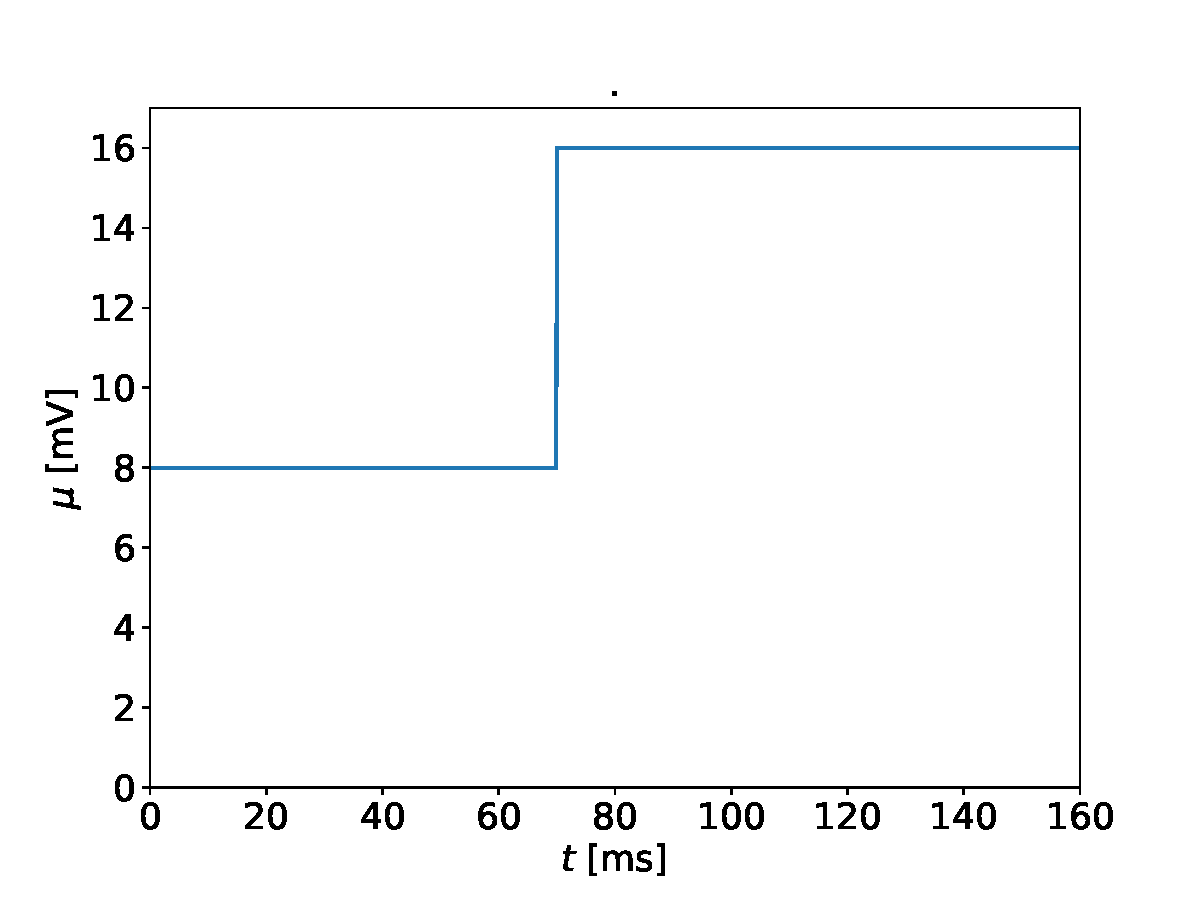
\includegraphics[width=70mm]{mu}
\end{figure}
\small{$V_{th}=15$ mV, $V_r=0$ mV, $\Delta = 2$ mV, $C=1000$ Hz, $\tau_m=20$ ms $dt=0.1$ ms, $N_{micro}=10^5$}
\end{frame}




\begin{frame}
\frametitle{1.2 The refractory density for a LIF neuron}
The activity is defined as:
$A(t)=q(0,t)=\int_{0}^{\infty}\rho(\tau,t)q(\tau,t)d\tau$

	\begin{figure}
	\centering
	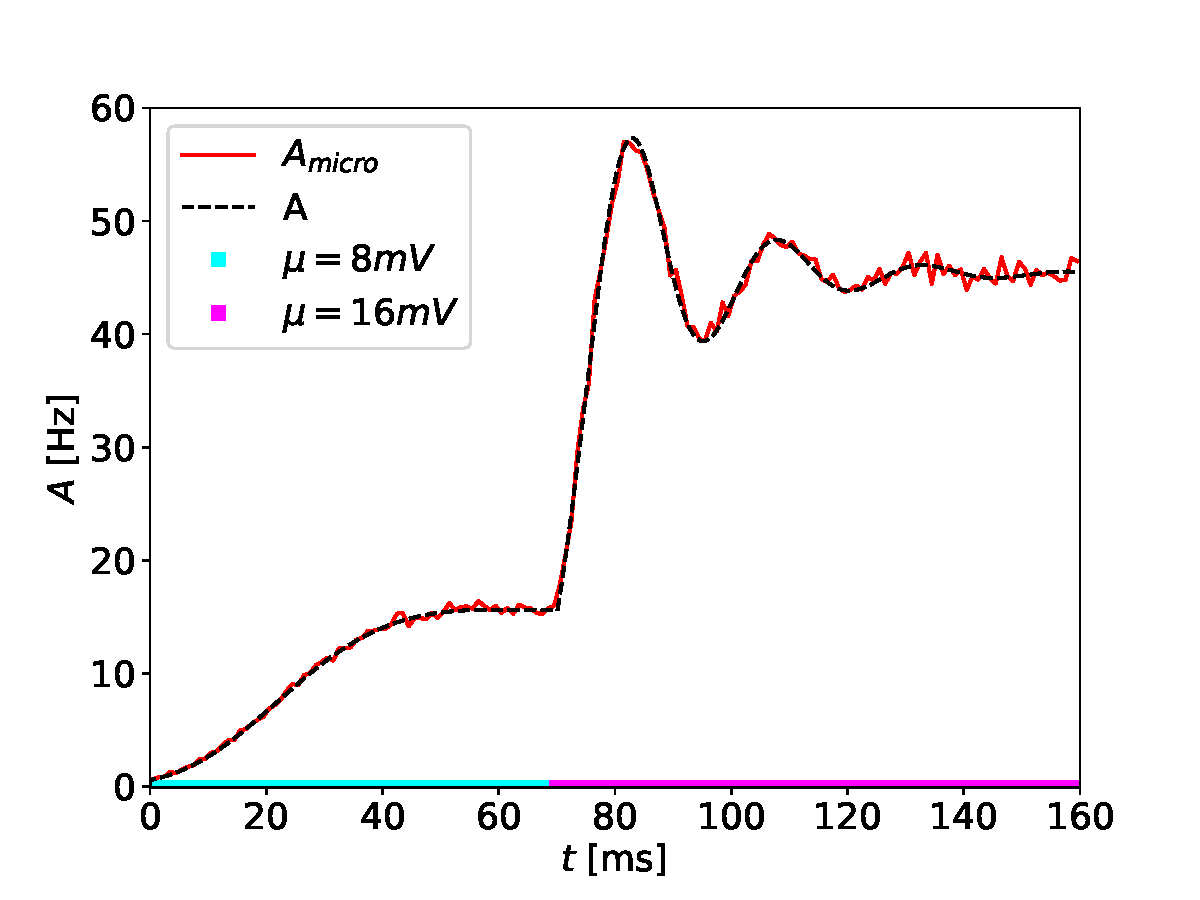
\includegraphics[width=8cm]{At_first}\   
\end{figure}

\small{$V_{th}=15$mV, $V_r=0$ mV, $\Delta = 2$ mV, $C=1000$ Hz, $\tau_m=20$ ms $dt=0.1$ ms, $N_{micro}=10^5$}

\end{frame}

\begin{frame}
\frametitle{Overview}% Table of contents slide, comment this block out to remove it
\tableofcontents % Throughout your presentation, if you choose to use \section{} and \subsection{} commands, these will automatically be printed on this slide as an overview of your presentation
\end{frame}


\section{2. Theoretical derivation}
\subsection{2.1 Eigenfunction expansion of the refractory density}

\begin{frame}
\frametitle{2. Theoretical derivation}
\framesubtitle{2.1 Eigenfunction expansion of the refractory density}

We consider first the time homogeneous case: $\rho(\tau,t)=\rho(\tau)$

\vspace{0.2cm}
\hspace{2.9cm}$
\partial_t q(\tau,t)=-\partial_\tau q(\tau,t)-\rho(\tau)q(\tau,t)=\mathcal{L}q(\tau,t)
$

\pause
\vspace{0.3cm}
We can expand the refractory density as:

\vspace{0.2cm}
\hspace{3.1cm}
$q(\tau,t)=\sum_n a_n(t)\phi_n(\tau) $

\pause
\vspace{0.3cm}
where $\phi_n(\tau)$ are the eigenfunctions of the operator 

\vspace{0.2cm}
 \hspace{1.2cm} $\mathcal{L}=-\partial_{\tau}-\rho(\tau)$ \hspace{1cm}$
\mathcal{L}\phi_n=\lambda_n\phi_n
$

\vspace{0.3cm}
With eigenvalues $\lambda_n$ and boundary conditions:
\begin{align}
\phi_n(0)&=\int_{0}^{\infty}\rho(\tau)\phi_n(\tau)d\tau \nonumber\\
\phi_n(\infty)&=0 \nonumber
\end{align}


\end{frame}


\begin{frame}
\frametitle{2. Eigenfunction expansion of the refractory density}

Solving $[-\partial_{\tau}-\rho(\tau)]\phi_n=\lambda_n\phi_n$ we have:

\vspace{0.2cm}

\hspace{1.8cm}$\phi_n(\tau)=\phi_n(0)\exp(-\lambda_n\tau-\int_0^\tau\rho(s)ds)$

\vspace{0.5cm}
\pause
Using the boundary condition we find:

\vspace{0.2cm}

\hspace{1.8cm}$\phi_n(0)=\int_0^{\infty}\rho(\tau)\phi_n(0)\exp(-\lambda_n\tau-\int_0^\tau\rho(s)ds)$

\vspace{0.5cm}
\pause
which can be written as:

\vspace{0.2cm}

\hspace{2.5cm}\fbox{$1=\int_0^{\infty}e^{-\lambda_n\tau}P(\tau)d\tau$}

\vspace{0.5cm}
with ISI density $P(\tau)=\rho(\tau) \exp(-\int_0^\tau\rho(s)ds)$

\vspace{0.5cm}
\pause
$\Rightarrow$ $\lambda_0=0$ fulfilled the condition, The eigenvalues must be complex, and the real part of $\lambda_n$ cannot be positive.


\end{frame}

\subsection{2.2 Definition and property of the adjoint operator $\mathcal{L}^+$}

\begin{frame}
\frametitle{2.2 Definition and property of the adjoint operator $\mathcal{L}^+$}

To recover the activity we will need the eigenfunctions $\psi_n$ of the adjoint operator $\mathcal{L}^+$:

\hspace{3.8cm}
$\mathcal{L}^+\psi_n=\lambda_n\psi_n$

\pause
\vspace{0.5cm}
Defining the inner product : $(\psi,\phi)=\int_{0}^{\infty}\psi(\tau)\phi(\tau)d\tau$

\vspace{0.5cm} and using the property: $(\psi,\mathcal{L}\phi)  = (\mathcal{L}^+\psi,\phi)$

\pause
\vspace{0.5cm} 
One can obtained the adjoint operator $\mathcal{L}^+$:


\vspace{0.2cm} 
\hspace{2cm}$
\mathcal{L}^+\psi(\tau)=[\partial_{\tau}-\rho(\tau)]\psi(\tau)+\psi(0)\rho(\tau)
$

\pause
\vspace{0.5cm} 
$\psi_n$, $\phi_n$ form a biorthonormal basis:
\vspace{0.3cm}
\hspace{3.8cm}
$
(\psi_i,\phi_j)=\delta_{ij}
$
\end{frame}





\subsection{2.3 Recover the Activity}
\begin{frame}
\frametitle{2.3 Recover the Activity}
The activity is given by:

\vspace{0.2cm}
\hspace{3cm} $A(t)=q(t,0)=\sum_n a_n(t)\phi_n(0) $

\pause
\vspace{0.5cm}
We derived $a_n(t)$ by projecting $q(\tau,t)$ on the eigenbasis:

\vspace{0.2cm}
\hspace{3cm}$ a_n(t)=(\psi_n,q)$

\pause
\vspace{0.5cm}
From which we obtained $\frac{d a_n}{dt}= \lambda_na_n$ and:

\vspace{0.2cm}
\hspace{3cm}$a_n(t) = a_n(0)\exp(\lambda_nt)$
%with \hspace{0.4cm} a_n(0) = & \int_{0}^{\infty}\psi_n(\tau)q(0,\tau)d\tau
%\end{align*}


\pause

\vspace{0.5cm}
Keeping the two first modes, one can obtain a second order differential equation for the firing rate :

\vspace{0.2cm}
\hspace{3cm}$\ddot A(t)=[2Re(\frac{1}{\lambda_1})\dot A(t)-A(t)+A_{\infty}] |{\lambda_1}|$

\vspace{0.2cm}
\small{M. Mattia, \textit{Low-dimensional firing rate dynamic of spiking neuron networks} (2016)}

%\pause
%\vspace{0.3cm}
%In particular for initial condition $q(0,\tau)=\delta(\tau)$ we have:

%\vspace{0.2cm}
%\hspace{3.8cm}$A(t)=\sum_n \psi_n(0)\phi_n(0)\exp(\lambda_nt) $

\end{frame}



\setbeamerfont{frametitle}{size=\Large}

\subsection{2.4 Resume of the theoretical derivation}
\begin{frame}
\frametitle{2.4 Resume of the theoretical derivation}

We can expand the refractory density as:

\vspace{0.2cm}
\hspace{3.1cm}
$q(\tau,t)=\sum_n a_n(t)\phi_n(\tau) $

\pause
\vspace{0.3cm}
from this expansion we found a condition for the eigenvalues $\lambda_n$:
\hspace{2.5cm}\fbox{$1=\int_0^{\infty}e^{-\lambda_n\tau}P(\tau)d\tau$}

\pause
\vspace{0.3cm}
Knowing the eigenvalues and the hazard function we can analytically define the eigenfunctions $\phi_n$ and $\psi_n$.

\pause
\vspace{0.3cm}
Thanks to those eigenfunctions we can recover the activity: %n particular starting with initial condition $q(0,\tau)=\delta(\tau)$ :

\vspace{0.2cm}
\hspace{3.cm}$A(t)=\sum_n a_n(t)\phi_n(0) $%$A(t)=\sum_n \psi_n(0)\phi_n(0)\exp(\lambda_nt) $

\end{frame}


\begin{frame}
\frametitle{Overview}% Table of contents slide, comment this block out to remove it
\tableofcontents % Throughout your presentation, if you choose to use \section{} and \subsection{} commands, these will automatically be printed on this slide as an overview of your presentation
\end{frame}

\section{3. Spectral expansion for different processes}

\subsection{3.1 LIF neuron with exponential link function}
\begin{frame}
\frametitle{3. Spectral expansion for different processes}
\framesubtitle{3.1 LIF neuron with exponential link function}
	In the case of the LIF neuron with exponential link function we can not find $\lambda_n$ from the condition:

	\vspace{0.2cm}
	\hspace{2.5cm}$1=\int_0^{\infty}e^{-\lambda_n\tau}P(\tau)d\tau$

\pause
	\vspace{0.7cm}	
	We can express the operator $\mathcal{L}$ in matrix form.
	
	And recover the activity computing the eigenvalues and eigenvectors of this matrix.
	
	
\end{frame}

\begin{frame}
\frametitle{3.1 LIF neuron with exponential link function}

\hspace{0.7cm}$\lambda_0=0\Rightarrow \partial_t q(\tau,t)=0$ \hspace{0.8cm} $A(t)=\sum_n \psi_n(0)\phi_n(0)\exp(\lambda_nt) $
\begin{figure}
	\centering
	\subfloat{
			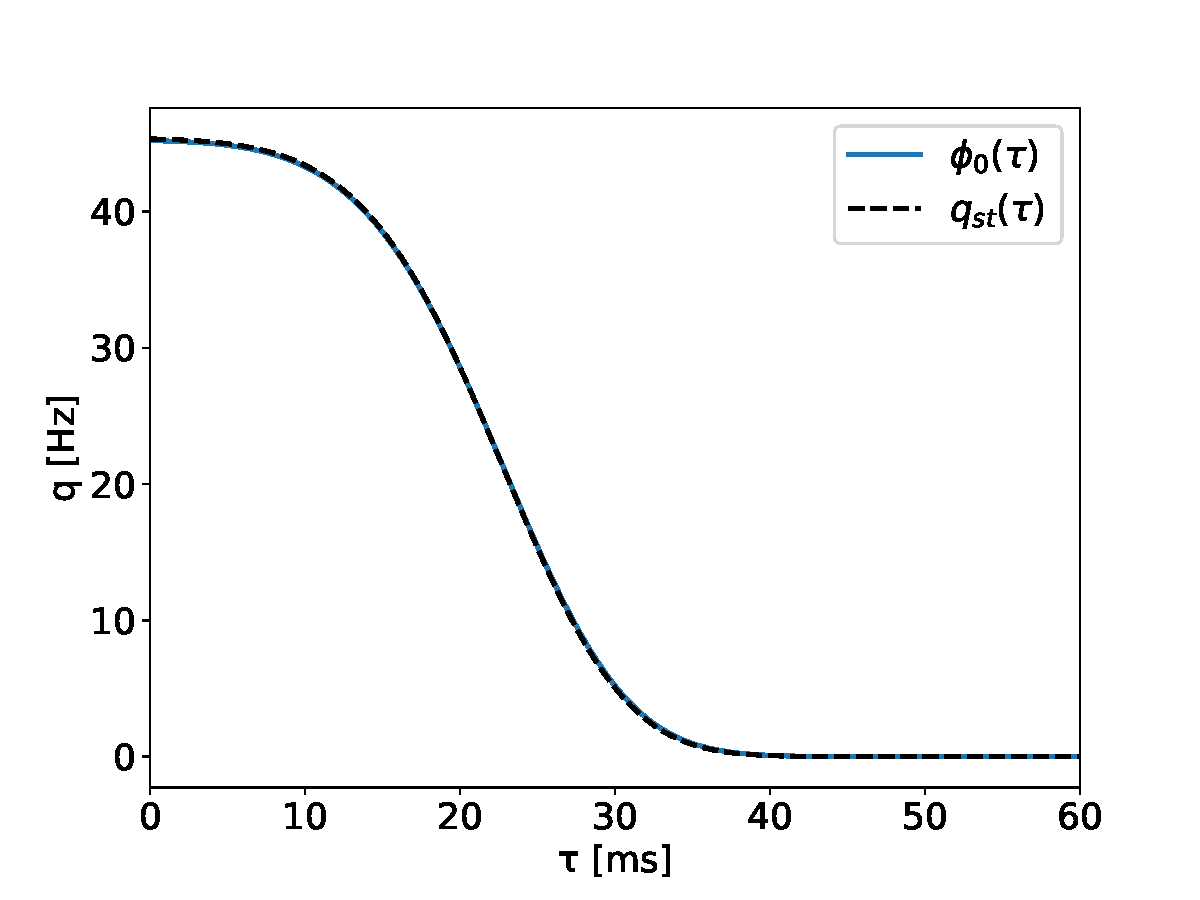
\includegraphics[width=55mm]{qfirst_st.pdf}
	
	}
	\subfloat{
		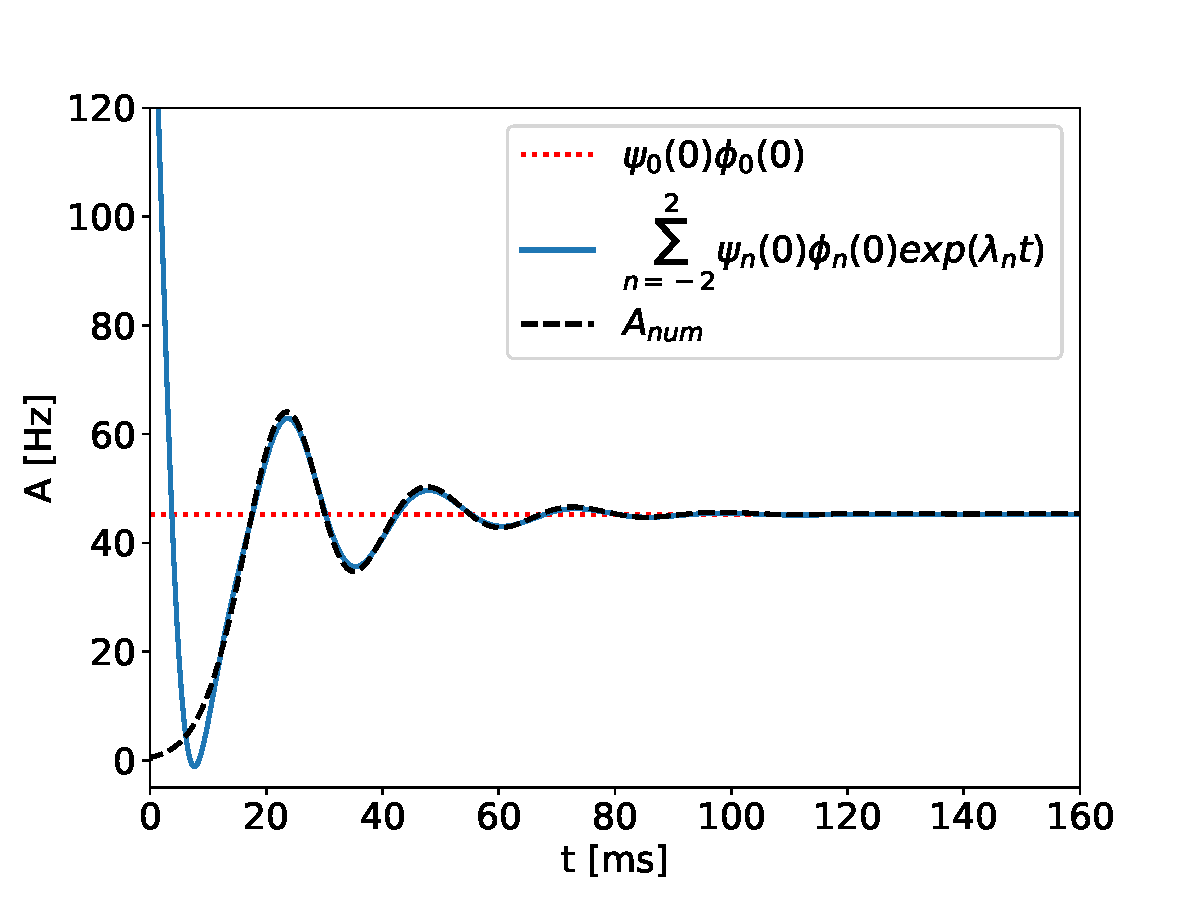
\includegraphics[width=55mm]{Amodefirst.pdf}
	}

\vspace{1cm}
\small{$\mu=16$ mV, $V_{th}=15$ mV, $V_r=0$ mV, $\Delta = 2$ mV, $C=1000$ Hz, $\tau_m=20$ ms $dt=0.1$ ms}
\end{figure}

\end{frame}




\subsection{3.2 Inverse Gaussian process}

\begin{frame}
\frametitle{3.2 Spectral expansion for different processes}
\framesubtitle{3.1 Inverse Gaussian process}
The perfect integrate fire model driven by a Gaussian white noise:

\vspace{0.3cm}
 $\dot V=\mu +\sqrt{2D}\xi(t)$ \hspace{1cm} $<\xi(t)\xi(s)>=\delta(t-s)$

\vspace{0.2cm}
 if $V=V_{th}:\:V\rightarrow V_r$
 
 \begin{figure}
 	\centering

 		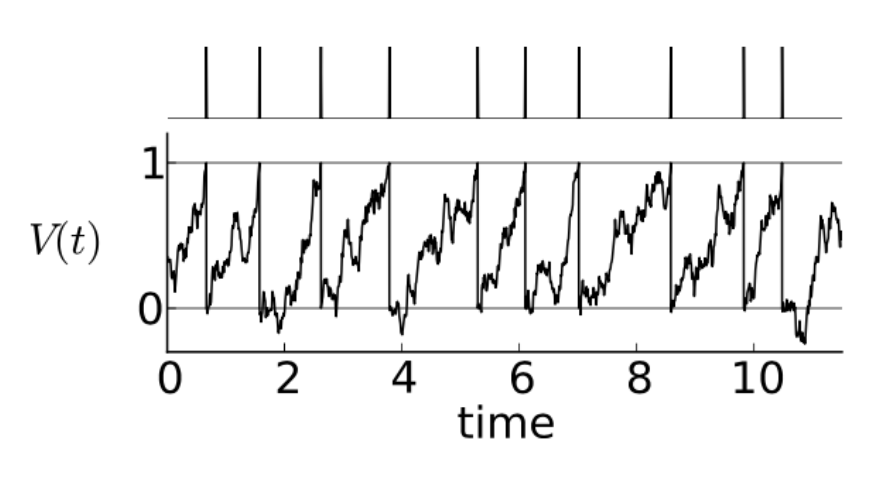
\includegraphics[width=70mm]{tilo}
 		
 		
 	\small{$\mu=1$, $D=0.125$ and $V_{th}=1$}\\
 	\tiny{
 	\textit{figure: T. Schwalger, The interspike-interval statistics of non-renewal neuron models (2013) }}
 	
 \end{figure}

\end{frame}

\begin{frame}
\frametitle{3.2 Inverse Gaussian process}
The ISI distribution is given by: 	

\vspace{0.2cm}
\hspace{2.5cm}$P(\tau)=\frac{V_{th}}{\sqrt{4\pi D\tau^3}}\exp(-\frac{(\mu\tau-V_{th})^2}{4D\tau})$


\pause
\vspace{0.3cm}
The Laplace transform can be derived analytically:

\vspace{0.2cm}
\hspace{2.5cm}$\bar{P}(\lambda)=\exp(\frac{\mu V_{th}}{2D}[1-\sqrt{1+\frac{4D\lambda}{\mu^2}}])$

\pause
\vspace{0.3cm}
Solving $\bar{P}(\lambda_n)=1$ we find:

\vspace{0.2cm}
\hspace{2.8cm} $\lambda_n=- \frac{2\pi\mu}{V_{th}}n( \frac{2\pi D}{\mu V_{th}}n + i)$



\end{frame}

\begin{frame}
\frametitle{3.2 Inverse Gaussian process}

Recover the activity solving the  second order differential equation:

\hspace{3cm} $\ddot A(t)=[2Re(\frac{1}{\lambda_1})\dot A(t)-A(t)+A_{\infty}] |{\lambda_1}|$

\begin{figure}
	\centering

		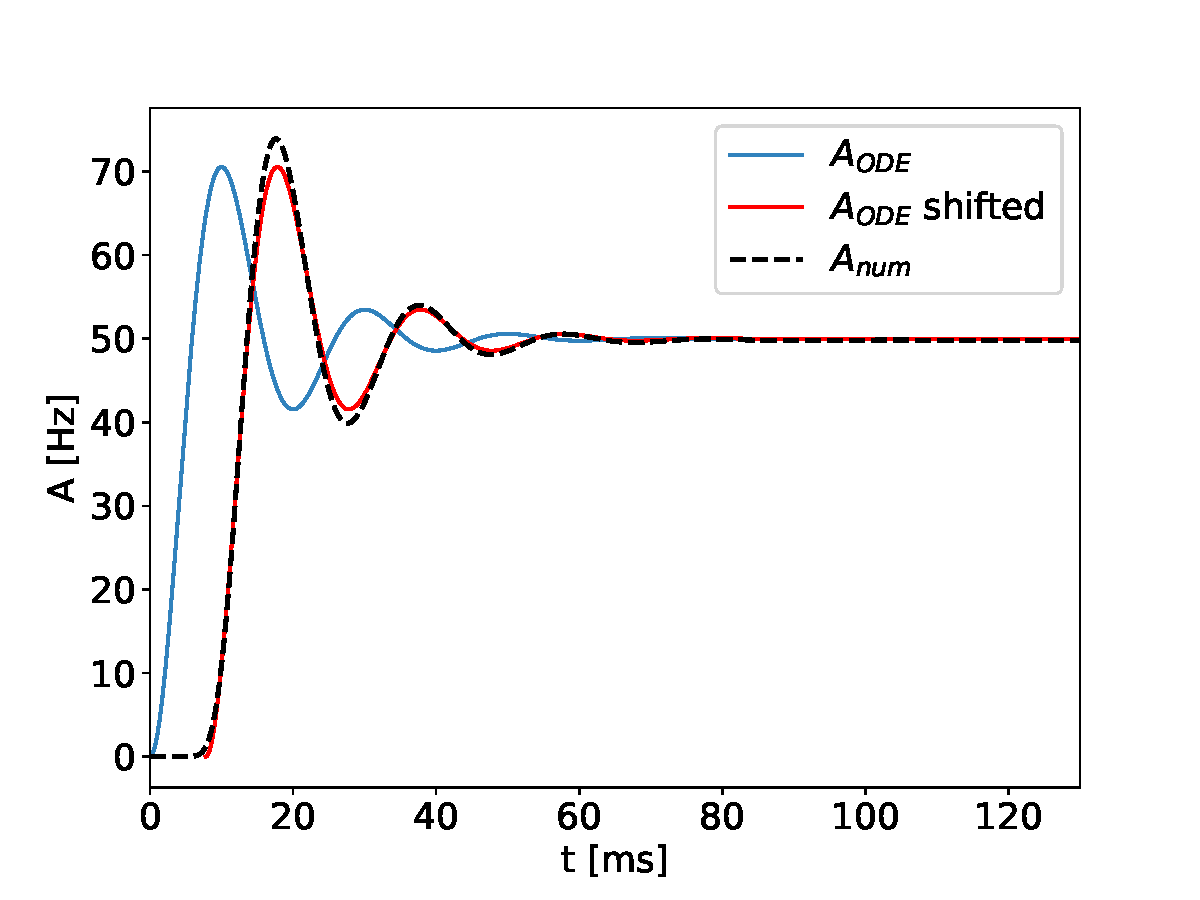
\includegraphics[width=70mm]{AODE.pdf}
			
	\vspace{0.5cm}
	\small{$\mu=50$ mV,$D=7.5$, $V_{th}=1$}
\end{figure}



\end{frame}

\begin{frame}
\frametitle{3.2 Inverse Gaussian process}
\hspace{0.7cm}$\lambda_0=0\Rightarrow \partial_t q(\tau,t)=0$ \hspace{0.8cm} $A(t)=\sum_n \psi_n(0)\phi_n(0)\exp(\lambda_nt) $
\begin{figure}
	\centering
	\subfloat{
		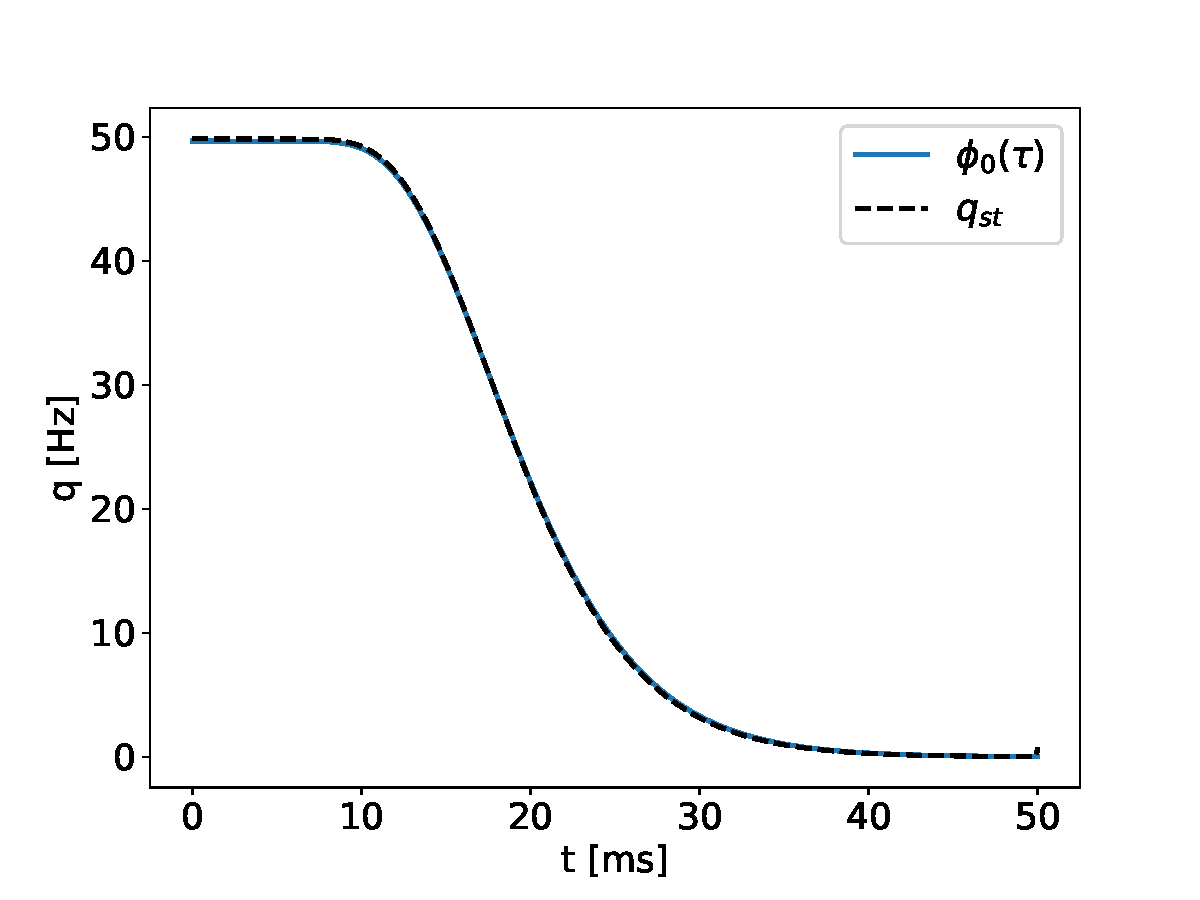
\includegraphics[width=55mm]{q_st.pdf}
		
	}
	\subfloat{
		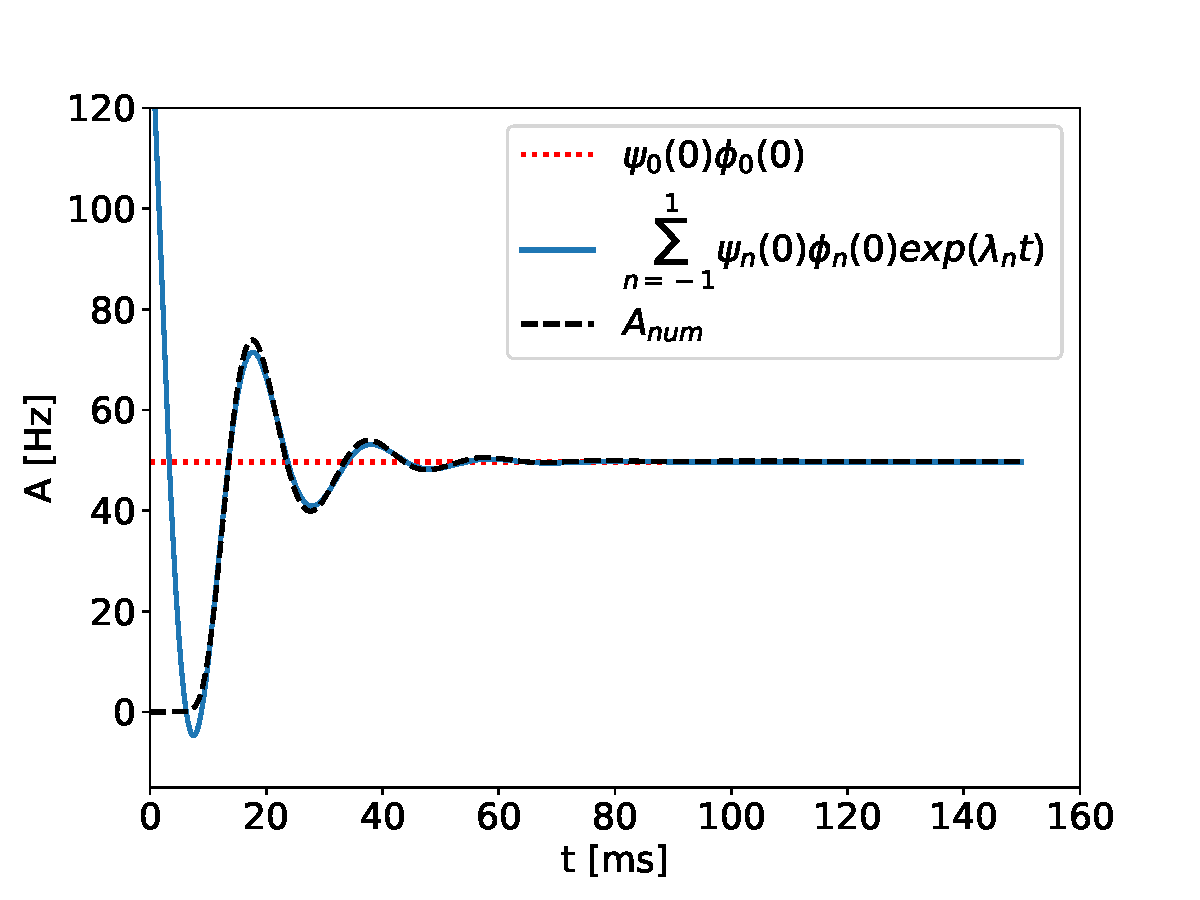
\includegraphics[width=55mm]{Amodefirst1.pdf}
	}
	
	\vspace{1cm}
	\small{$\mu=50$ mV,$D=7.5$, $V_{th}=1$}
\end{figure}

\end{frame}

\begin{frame}
\frametitle{3.2 Inverse Gaussian process}
Comparison of the theoretical spectrum and the eigenvalues obtained from the matrix form of $\mathcal{L}$
\begin{figure}
	\centering
	\subfloat{
		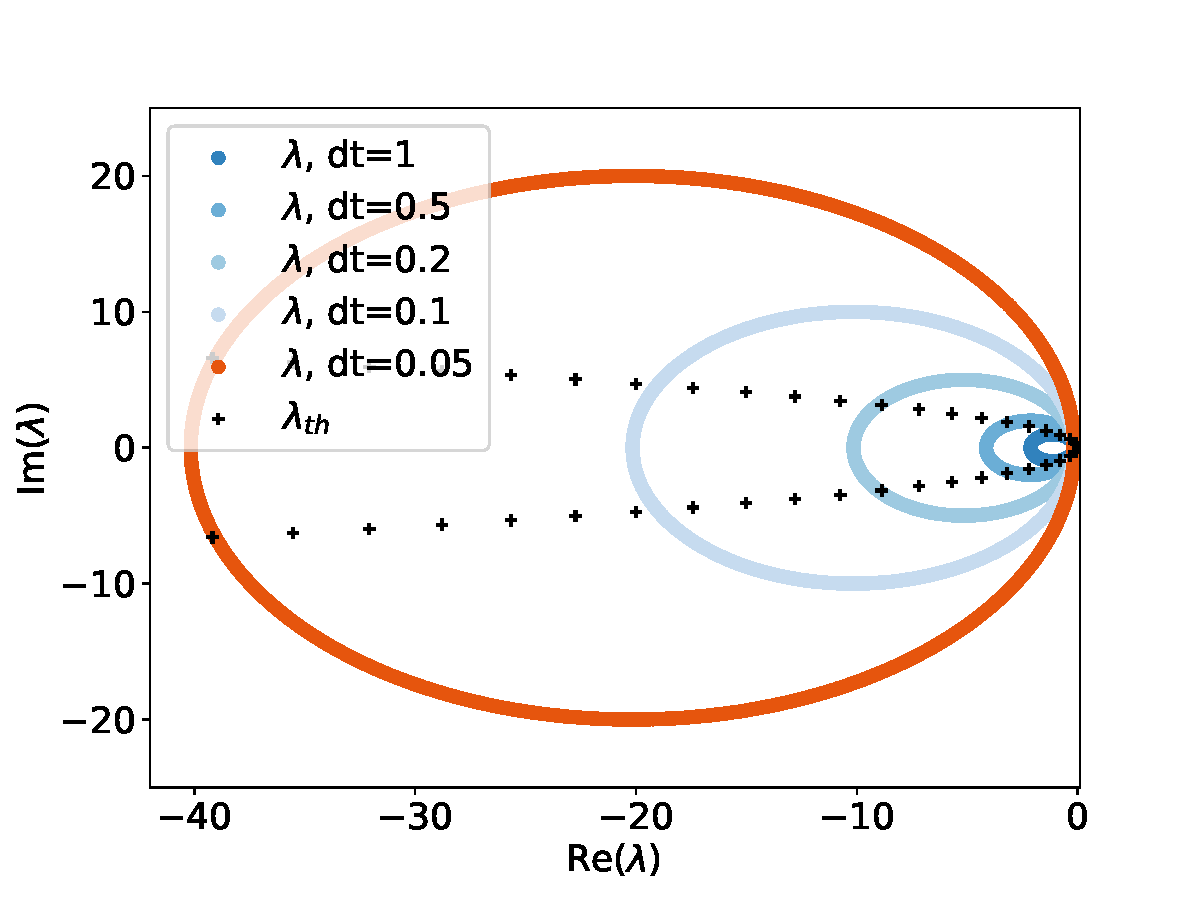
\includegraphics[width=45mm]{lambda_big.pdf}
		
	}
	\subfloat{
		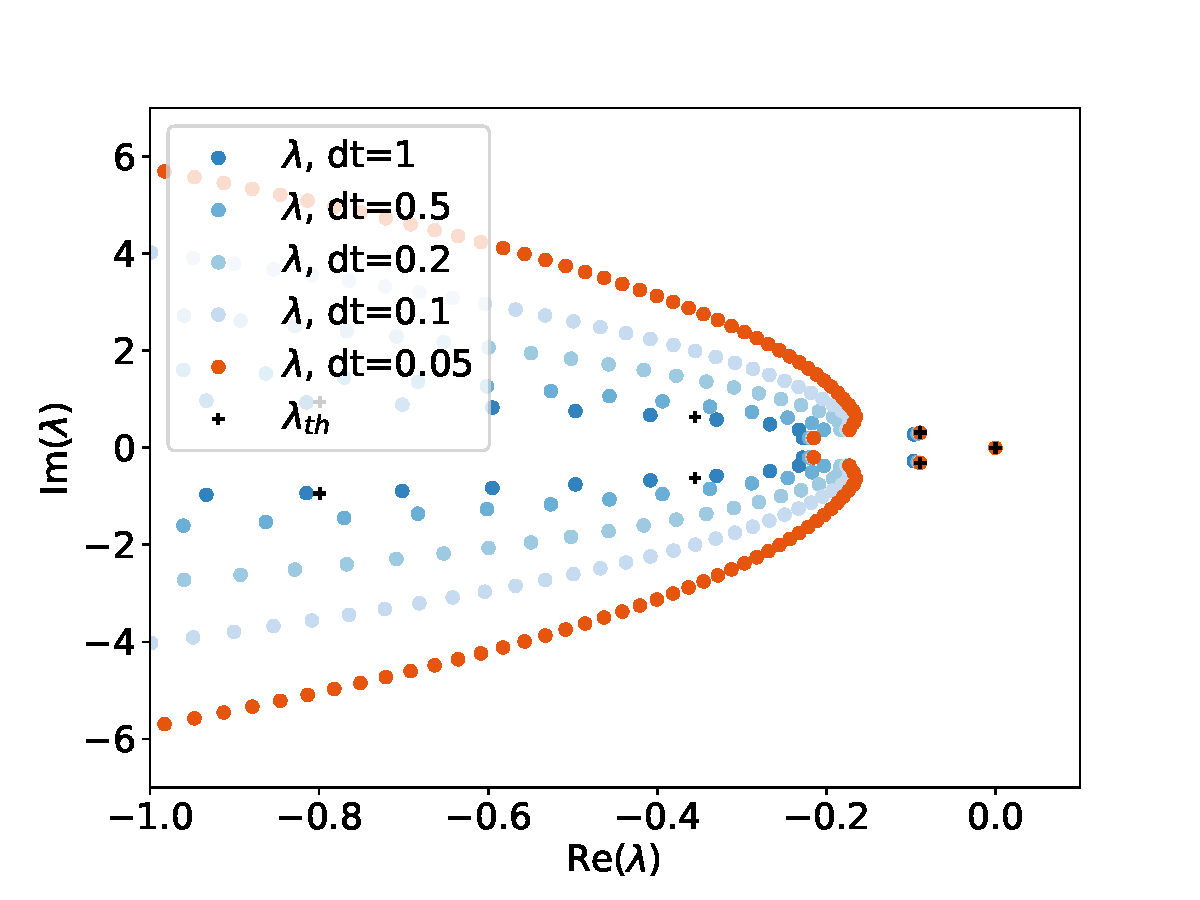
\includegraphics[width=45mm]{lambda.pdf}
	}\\
	\subfloat{
	
	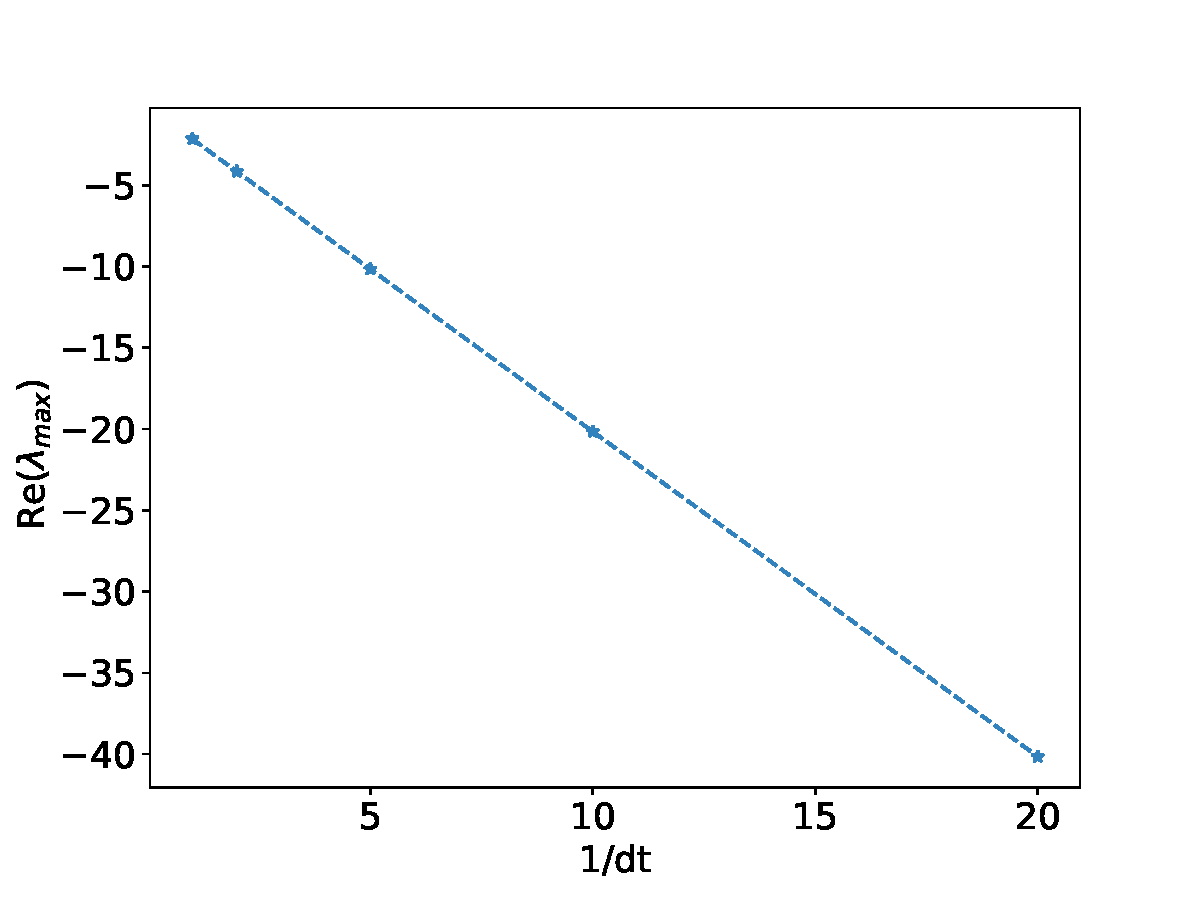
\includegraphics[width=45mm]{Re.pdf}
    }
	\subfloat{
	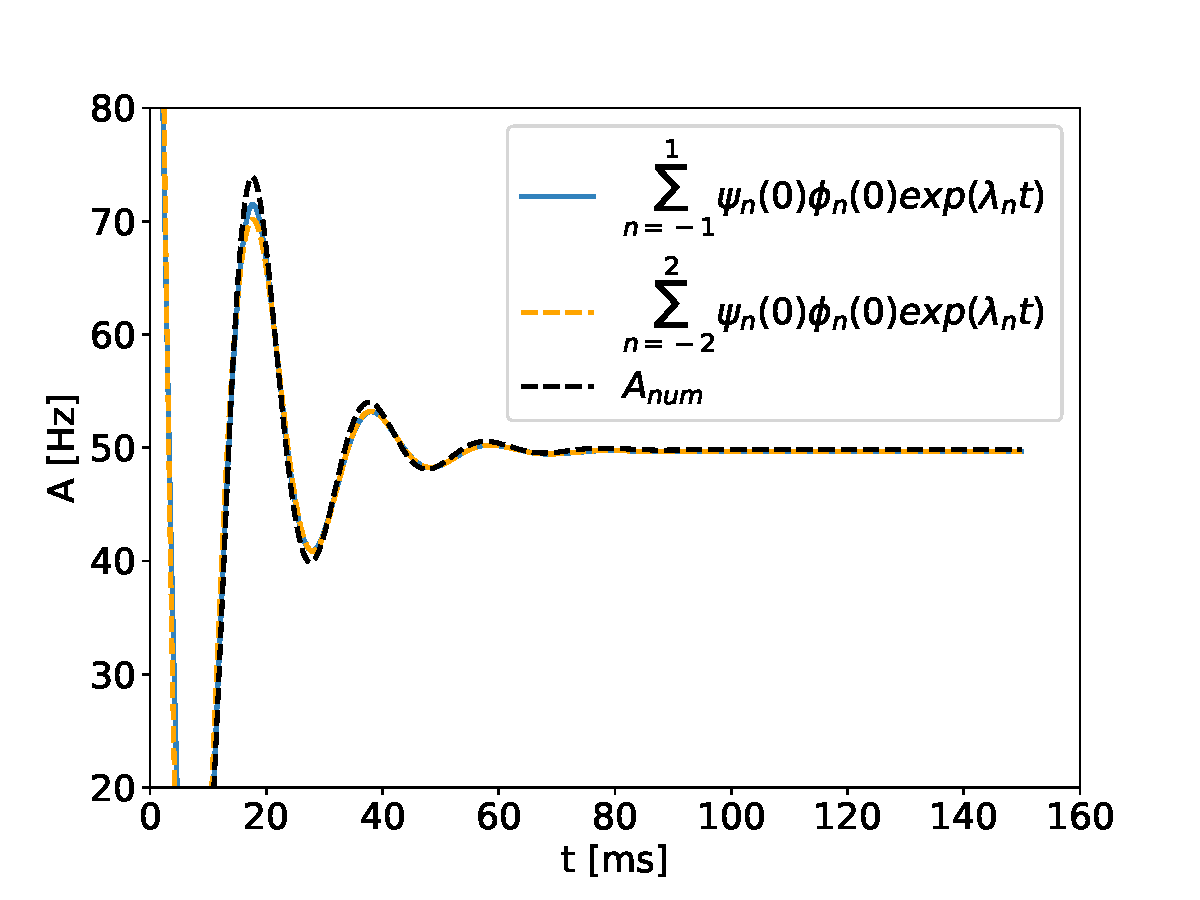
\includegraphics[width=45mm]{Amodefirst2.pdf}
}
	
	\vspace{1cm}
\end{figure}

\end{frame}

\subsection{3.3 Gamma process}
\begin{frame}
\frametitle{3.3 Gamma process}

The ISI distribution is given by: 	

\vspace{0.2cm}
\hspace{2.5cm}$P(\tau)=\frac{\beta^\gamma}{(\gamma-1)!}\tau^{\gamma-1}e^{-\beta\tau}$ for integer $\gamma$ and $\beta>0$. 

\pause
\vspace{0.3cm}
The Laplace transform can be derived analytically:

\vspace{0.2cm}
\hspace{2.5cm}$\bar{P}(\lambda)=(\frac{\beta}{\beta+\lambda})^\gamma$

\pause
\vspace{0.3cm}
Solving $\bar{P}(\lambda_n)=1$ we find:

\vspace{0.2cm}
\hspace{2.8cm} $\lambda_n=\beta(\exp(\frac{2\pi i}{\gamma}n)-1)$, $n=0,..., \gamma-1$

\end{frame}




\section{4. Summary and Future Work}
\begin{frame}
\begin{itemize}
	\frametitle{4. Summary and Future Work}
	\item 	We made an expansion of the refractory density for time homogeneous hazard rates $\rho(t,\tau)=\rho(\tau)$ 
	\pause
	\item We obtained a low dimensional dynamics for the firing rate in the case of uncoupled neuron
\end{itemize}
\pause
Future work:
\begin{itemize}
	
	\item Derive a low-dimensional ordinary differential equation for the firing rate in the case of a coupled network.
	
	\hspace{2cm} $\frac{d a_n}{dt}= \lambda_na_n+\frac{d\nu}{dt}(\frac{\partial \psi_n}{\partial \nu},q)$
	\pause
	\item Understand if there is an other constraint on the eigenvalues or if it's a numerical error. 


\end{itemize}




\end{frame}

\begin{frame}

\hspace{2cm} \Large{Thanks for your attention}

\end{frame}


%\subsection{3.2 Gamma process}




\begin{frame}
 one can show that for different eigenvalues, the eigenfunctions $\psi_i$ and $\phi_j$ are orthogonal:
\begin{align}
\lambda_j(\psi_i,\phi_j) 
&=(\psi_i,\mathcal{L}\phi_j) \nonumber \\
&=(\mathcal{L}^+\psi_i,\phi_j)  \nonumber \\
&=\lambda_i(\psi_i,\phi_j) \nonumber
\end{align}

\end{frame}


\begin{frame}
\frametitle{2.2 Definition and property of the adjoint operator $\mathcal{L}^+$}

\begin{align}
(\psi,\mathcal{L}\phi)&= \int_{0}^{\infty}\psi(\tau)\mathcal{L}\phi(\tau)d\tau  \nonumber \\
&= \int_{0}^{\infty}\psi(\tau)[-\partial_{\tau}-\rho(\tau)]\phi(\tau)d\tau  \nonumber \\
&=-[\psi(\tau)\phi(\tau)]^{\infty}_{0}+\int_{0}^{\infty}\partial_{\tau}\psi(\tau)\phi(\tau)d\tau -\int_{0}^{\infty}\rho(\tau)\psi(\tau)\phi(\tau)d\tau \nonumber \\
&= \psi(0)\phi(0)+ \int_{0}^{\infty}[\partial_{\tau}-\rho(\tau)]\psi(\tau)\phi(\tau)d\tau  \nonumber \\
&=\int_{0}^{\infty} \psi(0)\rho(\tau)\phi(\tau)d\tau+ \int_{0}^{\infty}[\partial_{\tau}-\rho(\tau)]\psi(\tau)\phi(\tau)d\tau  \nonumber \\
&= \int_{0}^{\infty}\{[\partial_{\tau}-\rho(\tau)]\psi(\tau)+ \psi(0)\rho(\tau)\}\phi(\tau)d\tau  \nonumber \\
& = (\mathcal{L}^+\psi,\phi) \nonumber
\end{align}

with 
$
\mathcal{L}^+\psi(\tau)=[\partial_{\tau}-\rho(\tau)]\psi(\tau)+\psi(0)\rho(\tau)
$
\end{frame}

\begin{frame}
\frametitle{2.2 Definition and property of the adjoint operator $\mathcal{L}^+$}
\begin{align*}
\mathcal{L}^+\psi_n(\tau)&=[\partial_{\tau}-\rho(\tau)]\psi_n(\tau)+\psi_n(0)\rho(\tau)\\
&=\lambda_n\psi_n(\tau)
\end{align*}

The solution of this equation is:

\vspace{0.2cm}

\begin{align*}
\psi_n(\tau)=&\psi_n(0)\exp(\lambda_n\tau+\int_0^\tau\rho(s)ds)\\
&-\psi_n(0)\int^\tau_0\rho(x)\exp\big{[}\lambda_n(\tau-x)+\int_0^{\tau-x}\rho(s)ds\big{]}dx
\end{align*}
\end{frame}

\begin{frame}
\frametitle{ Second order differential equation for the firing rate for uncoupled neurons}

\vspace{1cm}
M. Mattia, \textit{Low-dimensional firing rate dynamic of spiking neuron networks} (2016)

\vspace{1cm}

\hspace{1cm}$\ddot A(t)=[2Re(\frac{1}{\lambda_1})\dot A(t)-A(t)+A_{\infty}] |{\lambda_1}|$

\end{frame}


\end{document}